\begin{frame}
    \frametitle{Factoring, Classification}
\note{Filename: ccsd\_factoring06.tex}

\begin{block}{Diagram (2.26)} 
    \begin{equation*}
        \parbox{40mm}{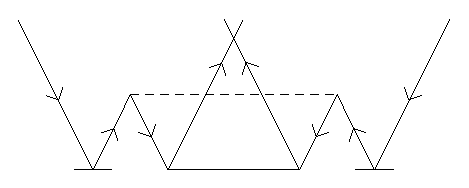
\includegraphics[scale=0.5]{graphics/ccsd_hbar_13_26}}
        = \frac{1}{4} P(ij) \bra{mn}\ket{ef} t_i^e t_{mn}^{ab} t_j^f
    \end{equation*}
\end{block}
This diagram is classified as $T_2(h^2) \times T_1(p) \times T_1(p)$
\begin{block}{Diagram (2.31)} 
    \begin{equation*}
        \parbox{40mm}{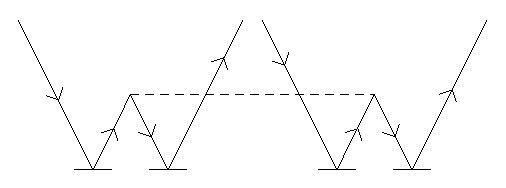
\includegraphics[scale=0.5]{graphics/ccsd_hbar_13_31}}
        = \frac{1}{4} P(ij) P(ab) \bra{mn}\ket{ef} t_i^e t_m^a t_j^f t_n^b
    \end{equation*}
\end{block}
This diagram is classified as $T_1(p) \times T_1(p) \times T_1(h) \times T_1(h)$
\end{frame}

